% Options for packages loaded elsewhere
% Options for packages loaded elsewhere
\PassOptionsToPackage{unicode}{hyperref}
\PassOptionsToPackage{hyphens}{url}
\PassOptionsToPackage{dvipsnames,svgnames,x11names}{xcolor}
%
\documentclass[
  letterpaper,
  DIV=11,
  numbers=noendperiod]{scrreprt}
\usepackage{xcolor}
\usepackage{amsmath,amssymb}
\setcounter{secnumdepth}{5}
\usepackage{iftex}
\ifPDFTeX
  \usepackage[T1]{fontenc}
  \usepackage[utf8]{inputenc}
  \usepackage{textcomp} % provide euro and other symbols
\else % if luatex or xetex
  \usepackage{unicode-math} % this also loads fontspec
  \defaultfontfeatures{Scale=MatchLowercase}
  \defaultfontfeatures[\rmfamily]{Ligatures=TeX,Scale=1}
\fi
\usepackage{lmodern}
\ifPDFTeX\else
  % xetex/luatex font selection
\fi
% Use upquote if available, for straight quotes in verbatim environments
\IfFileExists{upquote.sty}{\usepackage{upquote}}{}
\IfFileExists{microtype.sty}{% use microtype if available
  \usepackage[]{microtype}
  \UseMicrotypeSet[protrusion]{basicmath} % disable protrusion for tt fonts
}{}
\makeatletter
\@ifundefined{KOMAClassName}{% if non-KOMA class
  \IfFileExists{parskip.sty}{%
    \usepackage{parskip}
  }{% else
    \setlength{\parindent}{0pt}
    \setlength{\parskip}{6pt plus 2pt minus 1pt}}
}{% if KOMA class
  \KOMAoptions{parskip=half}}
\makeatother
% Make \paragraph and \subparagraph free-standing
\makeatletter
\ifx\paragraph\undefined\else
  \let\oldparagraph\paragraph
  \renewcommand{\paragraph}{
    \@ifstar
      \xxxParagraphStar
      \xxxParagraphNoStar
  }
  \newcommand{\xxxParagraphStar}[1]{\oldparagraph*{#1}\mbox{}}
  \newcommand{\xxxParagraphNoStar}[1]{\oldparagraph{#1}\mbox{}}
\fi
\ifx\subparagraph\undefined\else
  \let\oldsubparagraph\subparagraph
  \renewcommand{\subparagraph}{
    \@ifstar
      \xxxSubParagraphStar
      \xxxSubParagraphNoStar
  }
  \newcommand{\xxxSubParagraphStar}[1]{\oldsubparagraph*{#1}\mbox{}}
  \newcommand{\xxxSubParagraphNoStar}[1]{\oldsubparagraph{#1}\mbox{}}
\fi
\makeatother


\usepackage{longtable,booktabs,array}
\newcounter{none} % for unnumbered tables
\usepackage{calc} % for calculating minipage widths
% Correct order of tables after \paragraph or \subparagraph
\usepackage{etoolbox}
\makeatletter
\patchcmd\longtable{\par}{\if@noskipsec\mbox{}\fi\par}{}{}
\makeatother
% Allow footnotes in longtable head/foot
\IfFileExists{footnotehyper.sty}{\usepackage{footnotehyper}}{\usepackage{footnote}}
\makesavenoteenv{longtable}
\usepackage{graphicx}
\makeatletter
\newsavebox\pandoc@box
\newcommand*\pandocbounded[1]{% scales image to fit in text height/width
  \sbox\pandoc@box{#1}%
  \Gscale@div\@tempa{\textheight}{\dimexpr\ht\pandoc@box+\dp\pandoc@box\relax}%
  \Gscale@div\@tempb{\linewidth}{\wd\pandoc@box}%
  \ifdim\@tempb\p@<\@tempa\p@\let\@tempa\@tempb\fi% select the smaller of both
  \ifdim\@tempa\p@<\p@\scalebox{\@tempa}{\usebox\pandoc@box}%
  \else\usebox{\pandoc@box}%
  \fi%
}
% Set default figure placement to htbp
\def\fps@figure{htbp}
\makeatother


% definitions for citeproc citations
\NewDocumentCommand\citeproctext{}{}
\NewDocumentCommand\citeproc{mm}{%
  \begingroup\def\citeproctext{#2}\cite{#1}\endgroup}
\makeatletter
 % allow citations to break across lines
 \let\@cite@ofmt\@firstofone
 % avoid brackets around text for \cite:
 \def\@biblabel#1{}
 \def\@cite#1#2{{#1\if@tempswa , #2\fi}}
\makeatother
\newlength{\cslhangindent}
\setlength{\cslhangindent}{1.5em}
\newlength{\csllabelwidth}
\setlength{\csllabelwidth}{3em}
\newenvironment{CSLReferences}[2] % #1 hanging-indent, #2 entry-spacing
 {\begin{list}{}{%
  \setlength{\itemindent}{0pt}
  \setlength{\leftmargin}{0pt}
  \setlength{\parsep}{0pt}
  % turn on hanging indent if param 1 is 1
  \ifodd #1
   \setlength{\leftmargin}{\cslhangindent}
   \setlength{\itemindent}{-1\cslhangindent}
  \fi
  % set entry spacing
  \setlength{\itemsep}{#2\baselineskip}}}
 {\end{list}}
\usepackage{calc}
\newcommand{\CSLBlock}[1]{\hfill\break\parbox[t]{\linewidth}{\strut\ignorespaces#1\strut}}
\newcommand{\CSLLeftMargin}[1]{\parbox[t]{\csllabelwidth}{\strut#1\strut}}
\newcommand{\CSLRightInline}[1]{\parbox[t]{\linewidth - \csllabelwidth}{\strut#1\strut}}
\newcommand{\CSLIndent}[1]{\hspace{\cslhangindent}#1}



\setlength{\emergencystretch}{3em} % prevent overfull lines

\providecommand{\tightlist}{%
  \setlength{\itemsep}{0pt}\setlength{\parskip}{0pt}}



 


\KOMAoption{captions}{tableheading}
\makeatletter
\@ifpackageloaded{tcolorbox}{}{\usepackage[skins,breakable]{tcolorbox}}
\@ifpackageloaded{fontawesome5}{}{\usepackage{fontawesome5}}
\definecolor{quarto-callout-color}{HTML}{909090}
\definecolor{quarto-callout-note-color}{HTML}{0758E5}
\definecolor{quarto-callout-important-color}{HTML}{CC1914}
\definecolor{quarto-callout-warning-color}{HTML}{EB9113}
\definecolor{quarto-callout-tip-color}{HTML}{00A047}
\definecolor{quarto-callout-caution-color}{HTML}{FC5300}
\definecolor{quarto-callout-color-frame}{HTML}{acacac}
\definecolor{quarto-callout-note-color-frame}{HTML}{4582ec}
\definecolor{quarto-callout-important-color-frame}{HTML}{d9534f}
\definecolor{quarto-callout-warning-color-frame}{HTML}{f0ad4e}
\definecolor{quarto-callout-tip-color-frame}{HTML}{02b875}
\definecolor{quarto-callout-caution-color-frame}{HTML}{fd7e14}
\makeatother
\makeatletter
\@ifpackageloaded{bookmark}{}{\usepackage{bookmark}}
\makeatother
\makeatletter
\@ifpackageloaded{caption}{}{\usepackage{caption}}
\AtBeginDocument{%
\ifdefined\contentsname
  \renewcommand*\contentsname{Table of contents}
\else
  \newcommand\contentsname{Table of contents}
\fi
\ifdefined\listfigurename
  \renewcommand*\listfigurename{List of Figures}
\else
  \newcommand\listfigurename{List of Figures}
\fi
\ifdefined\listtablename
  \renewcommand*\listtablename{List of Tables}
\else
  \newcommand\listtablename{List of Tables}
\fi
\ifdefined\figurename
  \renewcommand*\figurename{Figure}
\else
  \newcommand\figurename{Figure}
\fi
\ifdefined\tablename
  \renewcommand*\tablename{Table}
\else
  \newcommand\tablename{Table}
\fi
}
\@ifpackageloaded{float}{}{\usepackage{float}}
\floatstyle{ruled}
\@ifundefined{c@chapter}{\newfloat{codelisting}{h}{lop}}{\newfloat{codelisting}{h}{lop}[chapter]}
\floatname{codelisting}{Listing}
\newcommand*\listoflistings{\listof{codelisting}{List of Listings}}
\makeatother
\makeatletter
\makeatother
\makeatletter
\@ifpackageloaded{caption}{}{\usepackage{caption}}
\@ifpackageloaded{subcaption}{}{\usepackage{subcaption}}
\makeatother
\usepackage{bookmark}
\IfFileExists{xurl.sty}{\usepackage{xurl}}{} % add URL line breaks if available
\urlstyle{same}
% fallback for those not using the hyperref driver hyperxmp:
\makeatletter
\@ifundefined{xmpquote}{\newcommand{\xmpquote}[1]{#1}}{}
\makeatother
\hypersetup{
  pdftitle={ds6400\_portfolio},
  pdfauthor={Samia Mahmood},
  colorlinks=true,
  linkcolor={blue},
  filecolor={Maroon},
  citecolor={Blue},
  urlcolor={Blue},
  pdfcreator={LaTeX via pandoc}}


\title{ds6400\_portfolio}
\author{Samia Mahmood}
\date{2026-08-27}
\begin{document}
\maketitle

\renewcommand*\contentsname{Table of contents}
{
\setcounter{tocdepth}{2}
\tableofcontents
}

\bookmarksetup{startatroot}

\chapter*{DS-6400: Advanced Machine Learning I
Portfolio}\label{ds-6400-advanced-machine-learning-i-portfolio}
\addcontentsline{toc}{chapter}{DS-6400: Advanced Machine Learning I
Portfolio}

\markboth{DS-6400: Advanced Machine Learning I Portfolio}{DS-6400:
Advanced Machine Learning I Portfolio}

This Quarto book will serve as my portfolio for DS-6400: Advanced
Machine Learning. Highlighting, my notes, propjects and presentaions.

To learn more about Quarto books visit
\url{https://quarto.org/docs/books}.

\bookmarksetup{startatroot}

\chapter{Introduction}\label{introduction}

This is a book created from markdown and executable code.

See Knuth (1984) for additional discussion of literate programming.

\bookmarksetup{startatroot}

\chapter{Simulation Study}\label{simulation-study}

\section{Paper Overview of Simulation Study (Efron
1983)}\label{paper-overview-of-simulation-study-efron-1983}

This section summarizes the simulation study discussed in Estimating the
Error Rate of a Prediction Rule: Improvement on Cross-Validation, (Efron
1983).

\begin{itemize}
\tightlist
\item
  \textbf{Title:} Estimating the Error Rate of a Prediction Rule:
  Improvement on Cross-Validation
\item
  \textbf{Author:} Bradley Efron
\item
  \textbf{Journal:} Journal of the American Statistical Association
\end{itemize}

\subsection{Central Goal of Study:}\label{central-goal-of-study}

\begin{itemize}
\tightlist
\item
  This study aims to build a prediction rule that classifies data into
  two classes using generated data and creates a prediction model and
  estimates the likelihood of that model making an incorrect prediction
  when tested on data it has never seen before. This is the true error
  rate. The study leverages statisical techniques such as cross
  validation, various bootstrapping methods, etc. and compares their
  error rates to determine which method gives the best estimate of the
  true error rate.
\end{itemize}

\subsection{Efron's Simulation Study
Step-by-Step:}\label{efrons-simulation-study-step-by-step}

\begin{enumerate}
\def\labelenumi{\arabic{enumi}.}
\tightlist
\item
  Efron uses a sampling experiment based on a specified probability
  model to generate artificial data for the simulation study.

  \begin{itemize}
  \tightlist
  \item
    For the sampling experiments such as the (2,14) sampling experiment,
    Efron generates data from a bivariate normal probability model with
    two predictor variables and two classes.
  \item
    The simulated dataset generates binary classes with equal
    probability of 50\% each:

    \begin{itemize}
    \tightlist
    \item
      \(P(Y = 0) = P(Y = 1) = 0.5\)
    \end{itemize}
  \item
    Where predictor vectors follow
    \href{bivariate_norm_dist.qmd}{class-conditional bivariate normal
    distributions}:

    \begin{itemize}
    \tightlist
    \item
      \(X \mid Y=0 \sim \mathcal{N}_2((-1,0)^T, \mathbf{I})\)
    \item
      \(X \mid Y=1 \sim \mathcal{N}_2((1,0)^T, \mathbf{I})\)
    \end{itemize}
  \end{itemize}
\item
  Efron uses the resulting training data to construct a classification
  rule using Fisher's linear discriminant. This prediction rule attempts
  to separate observations into their respective classes and is then
  used to predict the class of new observations.
\item
  In this simulation study, Efron has the apparant error rate which is
  used as a in-sample baseline to quantify optimism.
\item
  The specific method such as cross validation, bootstrapping, etc., is
  then used to test how well that classifier predicts unseen
  observations.
\item
  Efron then compares the error rates from the different methods like
  cross validation, bootstrapping, etc. and determines which method is
  the best estimator of the true error rate by calculating the MSE for
  each.

  \begin{itemize}
  \tightlist
  \item
    For a Single Trial (Trial \(i\) of 100) the estomated error rates
    for each method are:

    \begin{itemize}
    \tightlist
    \item
      \(\text{Err}_i\) (True Error Rate)
    \item
      \(\widehat{\text{Err}}_{i, \text{LOOCV}}\)
    \item
      \(\widehat{\text{Err}}_{i, \text{Boot}}\)
    \item
      \(\widehat{\text{Err}}_{i, \text{RBoot}}\)
    \item
      \(\widehat{\text{Err}}_{i, \text{SRBoot}}\)
    \item
      \(\widehat{\text{Err}}_{i, \text{DBoot}}\)
    \item
      \(\widehat{\text{Err}}_{i, \text{RDBoot}}\)
    \item
      \(\widehat{\text{Err}}_{i, .632}\)
    \end{itemize}
  \end{itemize}
\item
  He repeats this process 100 times, conducting 100 independent trials
  (generating 100 separate training datasets). For each trial, the true
  error rate (\(\text{Err}\)) and all estimated error rates
  (\(\widehat{\text{Err}}\)) are computed. The Mean Squared Error
  (\(\text{MSE}\)) is then calculated across these 100 trials to see
  which estimation method stays closest to the true error.
  \[\text{MSE}(\widehat{\text{Err}}) = \frac{1}{100} \sum_{i=1}^{100} \Big( \widehat{\text{Err}}_i - \text{Err}_i \Big)^2\]
\end{enumerate}

\section{Key Concepts}\label{key-concepts}

\subsection{Prediction Rule:}\label{prediction-rule}

\begin{itemize}
\tightlist
\item
  A Prediction rule is a specific decision threshold, score cutoff, or
  constraint derived from a model to classify subjects or take action.
\item
  In Efron's study, the prediction rule classifies data into two
  classes.

  \begin{itemize}
  \tightlist
  \item
    For example, whether a patient will ``survive'' or ``not survive''
  \item
    The mathematical representation is given by:
  \end{itemize}
\end{itemize}

\begin{tcolorbox}[enhanced jigsaw, arc=.35mm, bottomrule=.15mm, bottomtitle=1mm, breakable, colback=white, colbacktitle=quarto-callout-note-color!10!white, colframe=quarto-callout-note-color-frame, coltitle=black, left=2mm, leftrule=.75mm, opacityback=0, opacitybacktitle=0.6, rightrule=.15mm, title=\textcolor{quarto-callout-note-color}{\faInfo}\hspace{0.5em}{Definition: Indicator Loss}, titlerule=0mm, toprule=.15mm, toptitle=1mm]

The \textbf{Indicator Loss} function \(Q[y_i, \eta_i]\) measures whether
a model's prediction matches the true binary outcome:

\[
Q[y_i, \eta_i] = \begin{cases} 
0 & \text{if } \eta_i = y_i \\ 
1 & \text{if } \eta_i \neq y_i 
\end{cases}
\]

\begin{itemize}
\item
  \textbf{\(Q[y_i, \eta_i]\)} --- \textbf{Loss / Error Metric}\\
  Measures the accuracy or correctness of the prediction for the
  \(i\)-th individual observation.
\item
  \textbf{\(y_i\)} --- \textbf{True Response}\\
  The actual observed outcome for case \(i\) (e.g.,
  \(1 = \text{survive}\), \(0 = \text{not survive}\)).
\item
  \textbf{\(\eta_i\)} --- \textbf{Predicted Value}\\
  The value predicted by the model for case \(i\), where
  \(\eta_i = \eta(t_i, \mathbf{x})\).
\item
  \textbf{\(t_i\)} --- \textbf{Predictor Vector}\\
  The set of input features or covariates for case \(i\) (e.g., patient
  age, medical history).
\item
  \textbf{\(\mathbf{x}\)} --- \textbf{Training Set}\\
  The entire collection of training data
  \(\mathbf{x} = (x_1, x_2, \dots, x_n)\) used to construct the
  prediction rule \(\eta\).
\item
  \textbf{\(0 \text{ vs. } 1\)} --- \textbf{Indicator Loss}

  \begin{itemize}
  \tightlist
  \item
    \textbf{\(0\)}: Correct prediction (\(\eta_i = y_i\)). No error
    penalty.\\
  \item
    \textbf{\(1\)}: Misclassification (\(\eta_i \neq y_i\)). Standard
    binary classification error penalty.
  \end{itemize}
\end{itemize}

\end{tcolorbox}

\subsection{Error Rate:}\label{error-rate}

\begin{itemize}
\tightlist
\item
  True error rate \((Err)\) refers to the likelihood/probability of the
  model/prediction rule making the incorrect predicition when tested on
  data it was not trained on.
\end{itemize}

\begin{tcolorbox}[enhanced jigsaw, arc=.35mm, bottomrule=.15mm, bottomtitle=1mm, breakable, colback=white, colbacktitle=quarto-callout-note-color!10!white, colframe=quarto-callout-note-color-frame, coltitle=black, left=2mm, leftrule=.75mm, opacityback=0, opacitybacktitle=0.6, rightrule=.15mm, title=\textcolor{quarto-callout-note-color}{\faInfo}\hspace{0.5em}{Definition: True Error Rate}, titlerule=0mm, toprule=.15mm, toptitle=1mm]

The \textbf{True Error Rate (\(\text{Err}\))} is the expected loss when
applying the fixed prediction rule \(\eta(t, \mathbf{x})\) to an unseen,
randomly selected future observation \(X_0\):

\[
\text{Err} = E\Big[Q[Y_0, \eta(T_0, \mathbf{x})]\Big]
\]

\begin{itemize}
\item
  \textbf{\(\text{Err}\)} --- \textbf{True Error Rate}\\
  The theoretical out-of-sample error rate (generalization error) of the
  trained model on future unseen data.
\item
  \textbf{\(E[\,\cdot\,]\)} --- \textbf{Expectation Operator}\\
  The expected value (or probability of misclassification) evaluated
  over the true joint distribution of a new observation \((T_0, Y_0)\).
\item
  \textbf{\(X_0 = (T_0, Y_0)\)} --- \textbf{Unobserved Future Case}\\
  A new, independent data point drawn from the underlying distribution,
  consisting of predictor vector \(T_0\) and true response \(Y_0\).
\item
  \textbf{\(\eta(T_0, \mathbf{x})\)} --- \textbf{Model Prediction for
  Future Case}\\
  The prediction generated for predictor \(T_0\) using the fixed rule
  trained on dataset \(\mathbf{x}\).
\item
  \textbf{\(Q[\,\cdot\,,\,\cdot\,]\)} --- \textbf{Indicator Loss}\\
  Returns \(1\) if the prediction fails
  (\(\eta(T_0, \mathbf{x}) \neq Y_0\)) and \(0\) if correct.
\end{itemize}

\end{tcolorbox}

\begin{itemize}
\tightlist
\item
  Apparent error rate \((\bar{e}rr)\) refers to the
  likelihood/probability of the model/prediction rule making the
  incorrect predicition when tested on the same data it already trained
  on. The apparemnt error often gives misleading results that are too
  optimistic since the model has already ``seen the answer before'' so
  it did not actually ``learn the material.''
\end{itemize}

\begin{tcolorbox}[enhanced jigsaw, arc=.35mm, bottomrule=.15mm, bottomtitle=1mm, breakable, colback=white, colbacktitle=quarto-callout-note-color!10!white, colframe=quarto-callout-note-color-frame, coltitle=black, left=2mm, leftrule=.75mm, opacityback=0, opacitybacktitle=0.6, rightrule=.15mm, title=\textcolor{quarto-callout-note-color}{\faInfo}\hspace{0.5em}{Definition: Apparent Error Rate}, titlerule=0mm, toprule=.15mm, toptitle=1mm]

The \textbf{Apparent Error Rate (\(\bar{e}rr\))} is the empirical error
rate calculated by evaluating the prediction rule directly on the same
dataset used to train it:

\[
\bar{e}rr = \frac{1}{n} \sum_{i=1}^{n} Q[y_i, \eta(t_i, \mathbf{x})]
\]

\begin{itemize}
\item
  \textbf{\(\bar{e}rr\)} --- \textbf{Apparent Error Rate}\\
  The in-sample training error rate observed across the training set.
\item
  \textbf{\(n\)} --- \textbf{Sample Size}\\
  The total number of observations in the training set \(\mathbf{x}\).
\item
  \textbf{\(\sum_{i=1}^{n}\)} --- \textbf{Summation}\\
  Sums the loss across all individual training cases
  \(i = 1, 2, \dots, n\).
\item
  \textbf{\(y_i\)} --- \textbf{Observed Response}\\
  The actual response variable for the \(i\)-th training observation.
\item
  \textbf{\(\eta(t_i, \mathbf{x})\)} --- \textbf{In-Sample Prediction}\\
  The prediction made for training input \(t_i\) using the rule derived
  from training set \(\mathbf{x}\).
\item
  \textbf{\(\bar{e}rr < \text{Err}\)} --- \textbf{Optimism Bias}\\
  Because the same data is used both to fit and evaluate
  \(\eta(t, \mathbf{x})\), \(\bar{e}rr\) is typically overly optimistic
  (underestimates the true error).
\end{itemize}

\end{tcolorbox}

\begin{itemize}
\tightlist
\item
  Optimism (op) measures the diffference between the true error rate and
  the apparent error rate.
\end{itemize}

\begin{tcolorbox}[enhanced jigsaw, arc=.35mm, bottomrule=.15mm, bottomtitle=1mm, breakable, colback=white, colbacktitle=quarto-callout-note-color!10!white, colframe=quarto-callout-note-color-frame, coltitle=black, left=2mm, leftrule=.75mm, opacityback=0, opacitybacktitle=0.6, rightrule=.15mm, title=\textcolor{quarto-callout-note-color}{\faInfo}\hspace{0.5em}{Definition: Optimism}, titlerule=0mm, toprule=.15mm, toptitle=1mm]

The \textbf{Optimism (op)} is the random variable representing the
difference between the true error rate and the apparent error rate for a
given training set \(\mathbf{x}\): \[
\text{op} = \text{Err} - \bar{e}rr
\] The expected value of optimism over all possible training sets drawn
from distribution \(F\) is denoted by \(\omega(F)\):

\[
\omega(F) = E_F\{\text{op}(\mathbf{X}, F)\} = E_F\big\{\text{Err}(\mathbf{X}, F) - \bar{e}rr(\mathbf{X})\big\} \tag{2.5}
\]

\begin{itemize}
\item
  \textbf{\(\text{op}(\mathbf{x}, F)\)} --- \textbf{Optimism (Random
  Variable)}\\
  The realization of the gap between true generalization error and
  training error for a specific realized training dataset
  \(\mathbf{x}\).
\item
  \textbf{\(\omega(F)\)} --- \textbf{Expected Optimism}\\
  The theoretical average optimism over all datasets \(\mathbf{X}\)
  sampled from the population probability distribution \(F\).
\item
  \textbf{\(F\)} --- \textbf{True Data Generating Distribution}\\
  The underlying joint probability distribution of the data from which
  observations are sampled.
\item
  \textbf{\(\text{Err}(\mathbf{X}, F)\)} --- \textbf{True Error Rate}\\
  The expected loss of the model when applied to unseen future test
  cases sampled from \(F\).
\item
  \textbf{\(\bar{e}rr(\mathbf{X})\)} --- \textbf{Apparent Error Rate}\\
  The empirical error rate calculated directly on the training dataset
  \(\mathbf{X}\).
\item
  \textbf{\(E_F\{\,\cdot\,\}\)} --- \textbf{Expectation under \(F\)}\\
  The expected value taken over the random variation of the training
  dataset \(\mathbf{X}\) generated by distribution \(F\).
\end{itemize}

\end{tcolorbox}

\subsection{Fisher's Linear
Discriminant:}\label{fishers-linear-discriminant}

\begin{itemize}
\tightlist
\item
  Fisher's linear discriminant is a classification method used as a
  prediction rule where given an observation or data point, decide which
  group/class it belongs to.
\item
  Fisher's linear discriminat tries to find a linear boundary that
  separates the two classes as well as possible.
\item
  Efron utilzes the FIsher's linear discriminant as the prediction rule
  for this study.
\end{itemize}

\begin{figure}[H]

{\centering \pandocbounded{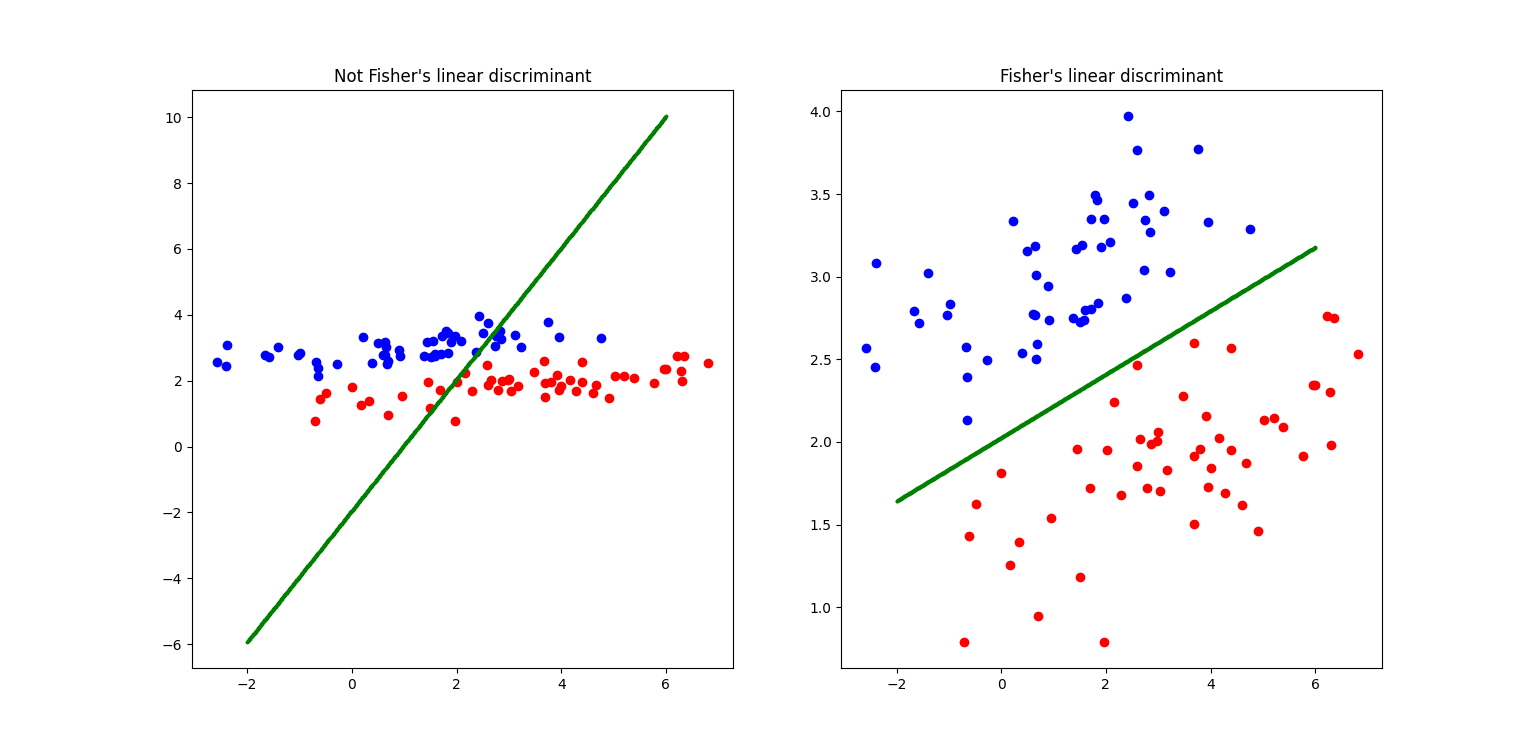
\includegraphics[keepaspectratio]{images/linear-discriminant.png}}

}

\caption{Figure 1: Visual for the Linear Discriminant.}

\end{figure}%

\subsection{Cross Validation:}\label{cross-validation}

\begin{itemize}
\tightlist
\item
  Cross-validation is a technique used to estimate how well a prediction
  model will perform on new, unseen data. It does this by dividing the
  available data into training and testing portions multiple times,
  fitting the model using the training portion, and evaluating its
  performance on the testing portion.
\item
  A fold of data refers to a chunk/subset of data.
\item
  The data is divided into k number equally-sized folds. During each
  iteration, k-1 number of folds of data are used for for training and
  the remaining 1 fold of data is used for testing. This is referred to
  a k-fold cross validation.
\item
  Cross Validation looks at the average of the performance scores from
  all iterations to get a final accuracy metric.
\item
  Cross Validation then compares the results across various models where
  each model sees the exact same folds to detmerine which model works
  best using the specific fold combination.
\end{itemize}

\begin{figure}[H]

{\centering \pandocbounded{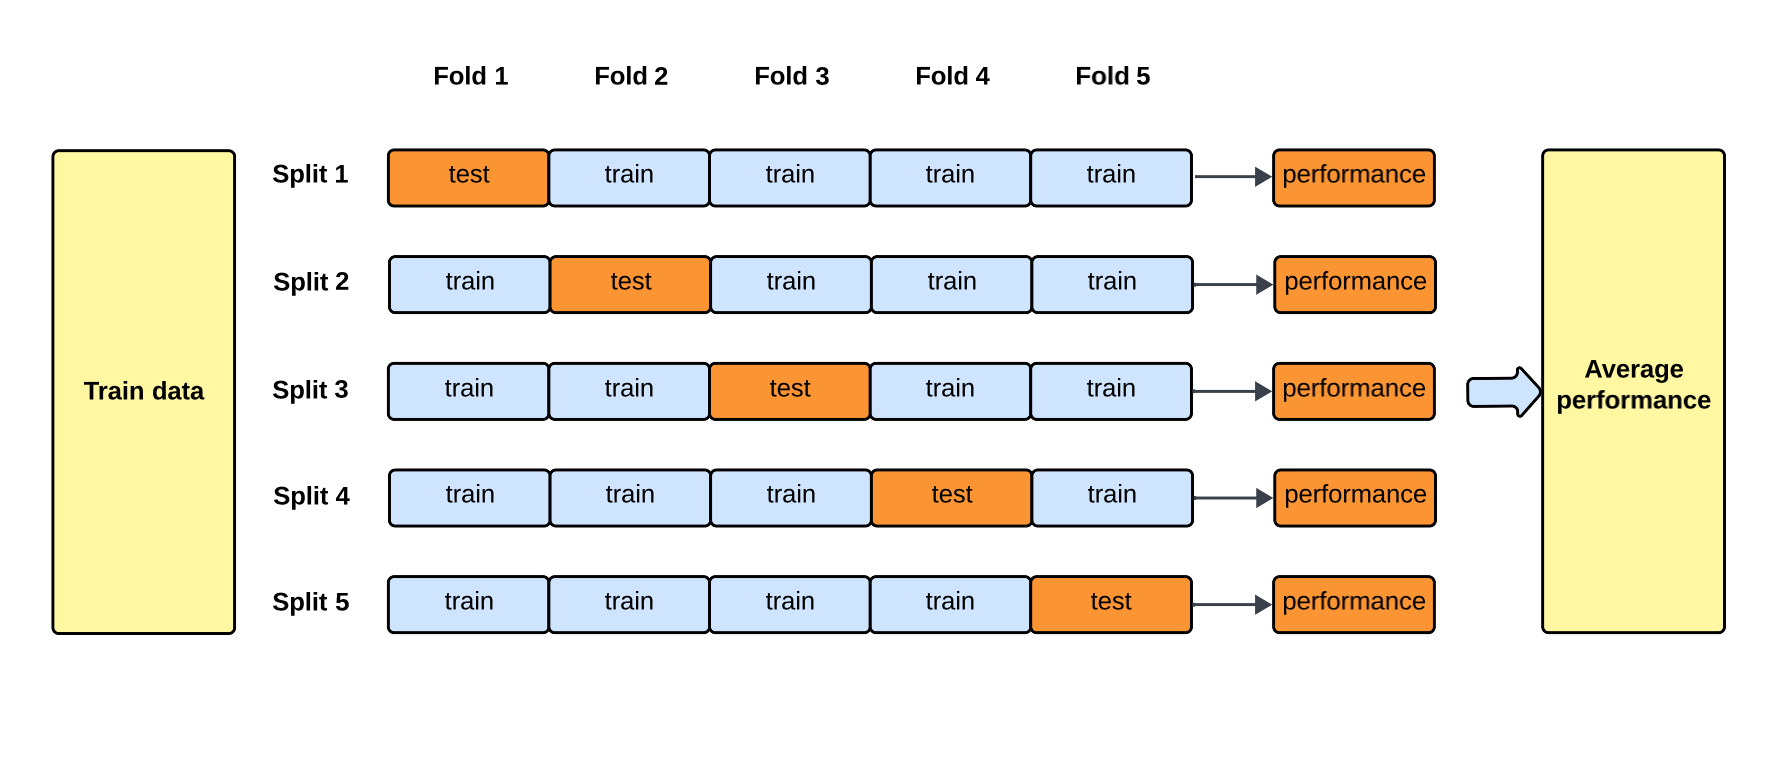
\includegraphics[keepaspectratio]{images/cross-validation.png}}

}

\caption{Figure 2: Diagram of Cross-Validation.}

\end{figure}%

\begin{itemize}
\tightlist
\item
  Additional information about Cross Validation can be referenced in the
  \href{cross_validation.qmd}{Cross Validation Chapter}.
\end{itemize}

\subsection{Bootstrapping:}\label{bootstrapping}

\begin{itemize}
\tightlist
\item
  Bootstrapping works by resampling a single dataset repeatedly with
  replacement (known as sampling with replacement) to estimate the
  variability, bias, or uncertainty of a statistic or estimator.
\item
  Bootstrapping takes a fixed original dataset of n number of
  observations.
\item
  Randomly draws a data points from the original dataset with
  replacement where a single data point from the original dataset may be
  picked more than once while some data points from the original dataset
  may not be picked at all.
\item
  This process is done until a new dataset is created known as the
  bootstrapped dataset with the same n number of data points as the
  original dataset.
\item
  This process is then repeated multiple times, producing multiple
  bootstrapped datasets.
\item
  The statisics for each of the bootstrapped datasets are taken.
\end{itemize}

\begin{figure}[H]

{\centering \pandocbounded{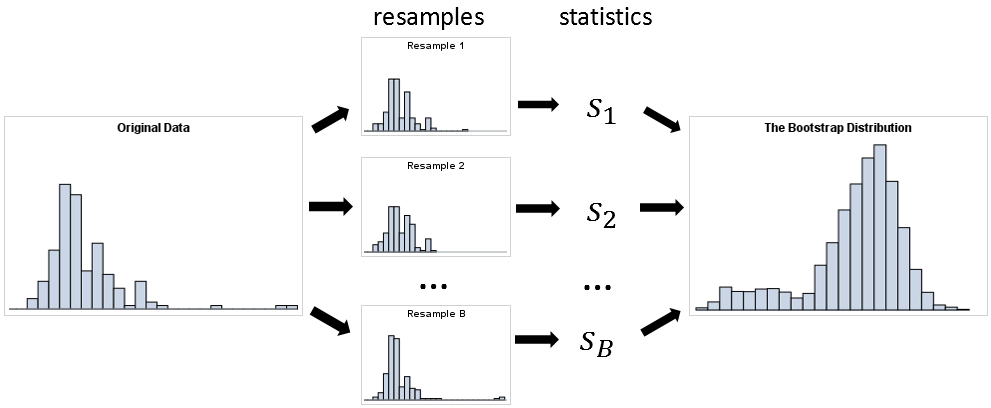
\includegraphics[keepaspectratio]{images/bootstrapping.png}}

}

\caption{Figure 3: Diagram of Bootstrapping.}

\end{figure}%

\begin{itemize}
\tightlist
\item
  Additional information about bootstrapping can be referenced in the
  \href{boostrapping.qmd}{Bootstrapping Chapter}.
\end{itemize}

\subsection{Mean Squared Error (MSE):}\label{mean-squared-error-mse}

\begin{itemize}
\tightlist
\item
  The MSE is the average of the squared differences between actual
  values and predicted values.
\item
  In Efron's study it is the squared difference between the true error
  rate and the estimated error rate. The formula used for the MSE for
  comparing both error rates is given by: \[
  MSE = E(\widehat{Err} - Err)^2
  \] Where: \[
  \widehat{Err} = \text{the estimated error rate}
  \] \[
  Err = \text{the true error rate}
  \]
\end{itemize}

\subsection{Bias Vs. Variance:}\label{bias-vs.-variance}

\begin{itemize}
\tightlist
\item
  Bias measures how far off a model's average predictions are from the
  correct values. Bias is the error from making oversimplified
  assumptions, leading to underfitting.

  \begin{itemize}
  \tightlist
  \item
    Underfitting refers to when the model is too simple to capture the
    underlying or key patterns in the data, resulting in poor
    performance on both training and testing datasets.
  \end{itemize}
\item
  Variance measures how much a model's predictions change if you train
  it on a different data subset. Variance is the error from the model
  being too sensitive to small changes in training data, leading to
  overfitting.

  \begin{itemize}
  \tightlist
  \item
    Overfitting refers to when the model learns the training data too
    well, is overly complex, sensitive, and flexible, resulting in the
    memorization of random noise and minor quirks instead of the true
    underlying or key patterns.
  \end{itemize}
\item
  For a good and reliable model, an optimal balance between simplicity
  and complexity, and thus, a low bias and low variance is required.

  \begin{itemize}
  \tightlist
  \item
    As model complexity increases, bias goes down and variance goes up.
  \item
    As model simplicity increases, bias goes up and variance goes down.
  \end{itemize}
\end{itemize}

\begin{figure}[H]

{\centering \pandocbounded{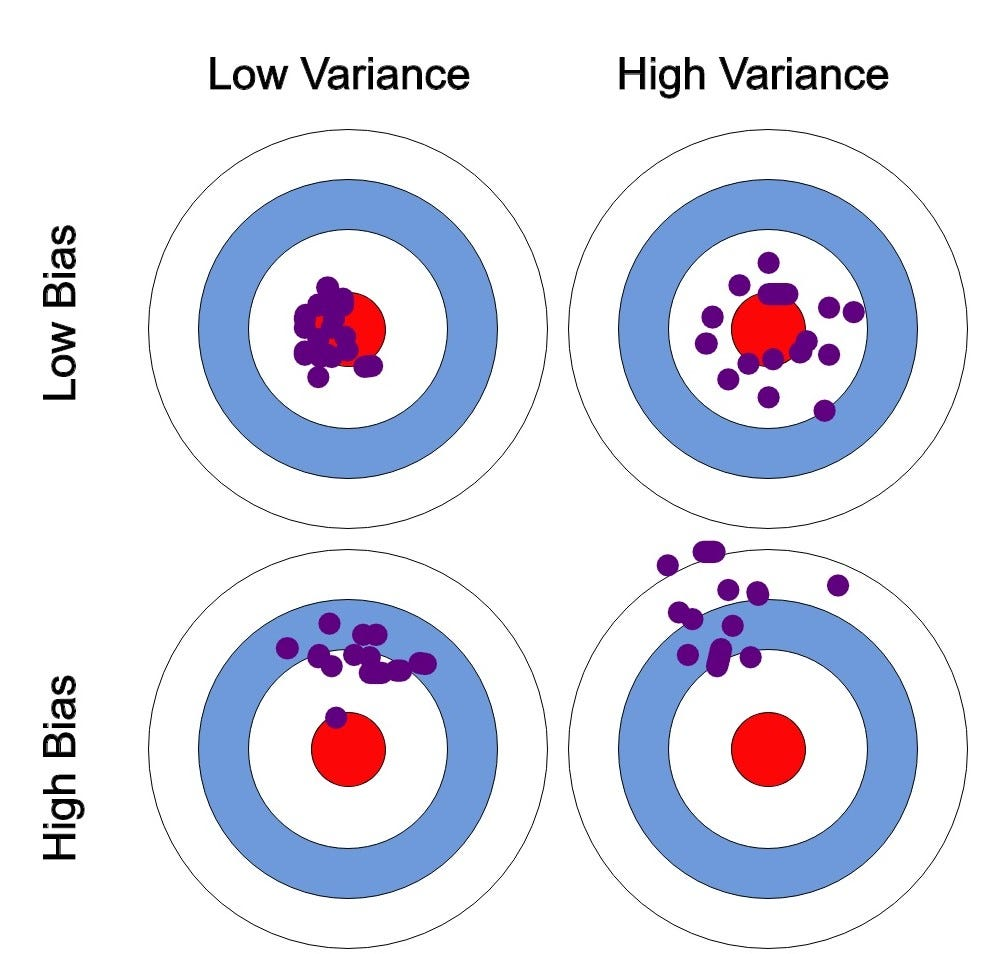
\includegraphics[keepaspectratio]{images/bias-variance-relation.jpeg}}

}

\caption{Figure 4: Diagram depicting relationship between bias and
variance.}

\end{figure}%

\begin{figure}[H]

{\centering \pandocbounded{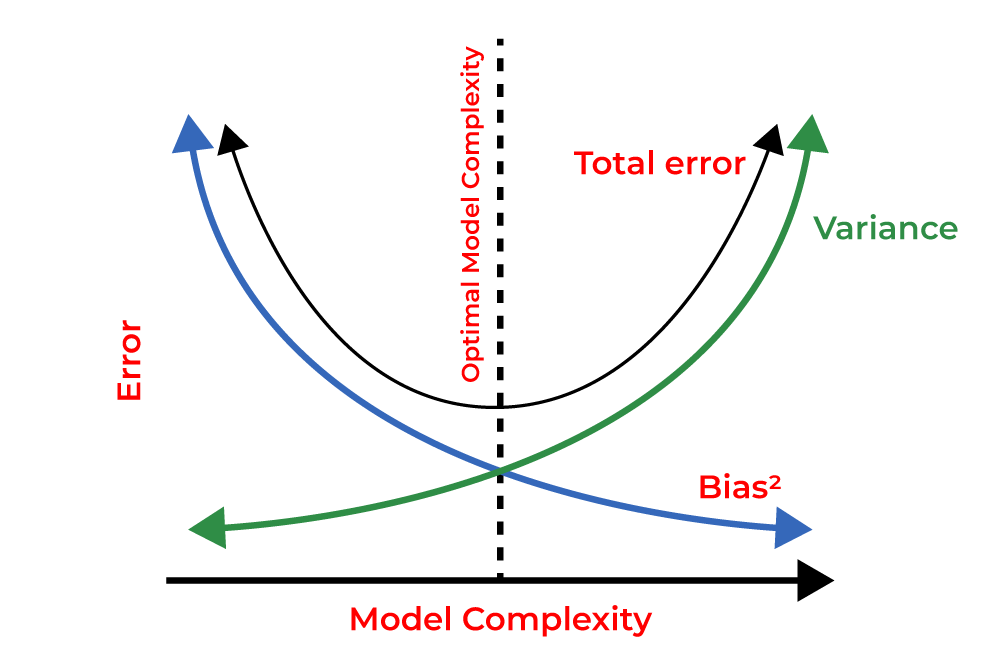
\includegraphics[keepaspectratio]{images/bias-variance-simplicity-complexity-graph.png}}

}

\caption{Figure 5: Graph displahying the relation between bias and
variance as model complexity changes.}

\end{figure}%

\section{Simulation Study Procedure Defined in Efron
1983}\label{simulation-study-procedure-defined-in-efron-1983}

\subsection{Sampling Experiements
Used:}\label{sampling-experiements-used}

\begin{itemize}
\tightlist
\item
  \textbf{Sampling Experiment \#1 - (2, 14):}

  \begin{itemize}
  \tightlist
  \item
    2 predictors - 2 independent variables
  \item
    14 observations - sample size of 14
  \item
    100 trials - the experiement was repreated 100 times
  \item
    For example: visualize the data as a matrix
  \end{itemize}

  {\def\LTcaptype{none} % do not increment counter
  \begin{longtable}[]{@{}lrrl@{}}
  \toprule\noalign{}
  Observation & Variable 1 \((X_1)\) & Variable 2 \((X_2)\) & Class
  \((Y)\) \\
  \midrule\noalign{}
  \endhead
  \bottomrule\noalign{}
  \endlastfoot
  1 & 22 & 35 & A \\
  2 & 31 & 52 & B \\
  3 & 27 & 41 & A \\
  \ldots{} & \ldots{} & \ldots{} & \ldots{} \\
  14 & 45 & 75 & B \\
  \end{longtable}
  }
\item
  \textbf{Sampling Experiment \#2 - (2, 20):}

  \begin{itemize}
  \tightlist
  \item
    2 predictors - 2 independent variables
  \item
    20 observations - sample size of 20 (allows Efron to see what
    happens when sample size increases)
  \item
    100 trials - the experiement was repreated 100 times
  \item
    For example: visualize the data as a matrix
  \end{itemize}

  {\def\LTcaptype{none} % do not increment counter
  \begin{longtable}[]{@{}lrrl@{}}
  \toprule\noalign{}
  Observation & Variable 1 \((X_1)\) & Variable 2 \((X_2)\) & Class
  \((Y)\) \\
  \midrule\noalign{}
  \endhead
  \bottomrule\noalign{}
  \endlastfoot
  1 & 22 & 35 & A \\
  2 & 31 & 52 & B \\
  3 & 27 & 41 & A \\
  \ldots{} & \ldots{} & \ldots{} & \ldots{} \\
  20 & 56 & 67 & A \\
  \end{longtable}
  }
\item
  \textbf{Sampling Experiment \#3 -(5, 14):}

  \begin{itemize}
  \tightlist
  \item
    5 predictors - 5 independent variables (allows Efron to see what
    happens when the number of predictors increase)
  \item
    14 observations - sample size of 14
  \item
    100 trials - the experiement was repreated 100 times
  \item
    For example: visualize the data as a matrix
  \end{itemize}

  {\def\LTcaptype{none} % do not increment counter
  \begin{longtable}[]{@{}
    >{\raggedright\arraybackslash}p{(\linewidth - 12\tabcolsep) * \real{0.2157}}
    >{\raggedleft\arraybackslash}p{(\linewidth - 12\tabcolsep) * \real{0.1373}}
    >{\raggedleft\arraybackslash}p{(\linewidth - 12\tabcolsep) * \real{0.1373}}
    >{\raggedleft\arraybackslash}p{(\linewidth - 12\tabcolsep) * \real{0.1373}}
    >{\raggedleft\arraybackslash}p{(\linewidth - 12\tabcolsep) * \real{0.1373}}
    >{\raggedleft\arraybackslash}p{(\linewidth - 12\tabcolsep) * \real{0.1373}}
    >{\raggedright\arraybackslash}p{(\linewidth - 12\tabcolsep) * \real{0.0980}}@{}}
  \toprule\noalign{}
  \begin{minipage}[b]{\linewidth}\raggedright
  Observation
  \end{minipage} & \begin{minipage}[b]{\linewidth}\raggedleft
  \((X_1)\)
  \end{minipage} & \begin{minipage}[b]{\linewidth}\raggedleft
  \((X_2)\)
  \end{minipage} & \begin{minipage}[b]{\linewidth}\raggedleft
  \((X_3)\)
  \end{minipage} & \begin{minipage}[b]{\linewidth}\raggedleft
  \((X_4)\)
  \end{minipage} & \begin{minipage}[b]{\linewidth}\raggedleft
  \((X_5)\)
  \end{minipage} & \begin{minipage}[b]{\linewidth}\raggedright
  Class
  \end{minipage} \\
  \midrule\noalign{}
  \endhead
  \bottomrule\noalign{}
  \endlastfoot
  1 & \ldots{} & \ldots{} & \ldots{} & \ldots{} & \ldots{} & A \\
  2 & \ldots{} & \ldots{} & \ldots{} & \ldots{} & \ldots{} & B \\
  3 & \ldots{} & \ldots{} & \ldots{} & \ldots{} & \ldots{} & A \\
  \ldots{} & \ldots{} & \ldots{} & \ldots{} & \ldots{} & \ldots{} &
  \ldots{} \\
  14 & \ldots{} & \ldots{} & \ldots{} & \ldots{} & \ldots{} & A \\
  \end{longtable}
  }
\item
  \textbf{Sampling Experiment \#4 - (5, 20):}

  \begin{itemize}
  \tightlist
  \item
    5 predictors - 5 independent variables (allows Efron to see what
    happens when the number of predictors increase)
  \item
    20 observations - sample size of 20 (allows Efron to see what
    happens when sample size increases)
  \item
    100 trials - the experiement was repreated 100 times
  \item
    For example: visualize the data as a matrix
  \end{itemize}

  {\def\LTcaptype{none} % do not increment counter
  \begin{longtable}[]{@{}
    >{\raggedright\arraybackslash}p{(\linewidth - 12\tabcolsep) * \real{0.2157}}
    >{\raggedleft\arraybackslash}p{(\linewidth - 12\tabcolsep) * \real{0.1373}}
    >{\raggedleft\arraybackslash}p{(\linewidth - 12\tabcolsep) * \real{0.1373}}
    >{\raggedleft\arraybackslash}p{(\linewidth - 12\tabcolsep) * \real{0.1373}}
    >{\raggedleft\arraybackslash}p{(\linewidth - 12\tabcolsep) * \real{0.1373}}
    >{\raggedleft\arraybackslash}p{(\linewidth - 12\tabcolsep) * \real{0.1373}}
    >{\raggedright\arraybackslash}p{(\linewidth - 12\tabcolsep) * \real{0.0980}}@{}}
  \toprule\noalign{}
  \begin{minipage}[b]{\linewidth}\raggedright
  Observation
  \end{minipage} & \begin{minipage}[b]{\linewidth}\raggedleft
  \((X_1)\)
  \end{minipage} & \begin{minipage}[b]{\linewidth}\raggedleft
  \((X_2)\)
  \end{minipage} & \begin{minipage}[b]{\linewidth}\raggedleft
  \((X_3)\)
  \end{minipage} & \begin{minipage}[b]{\linewidth}\raggedleft
  \((X_4)\)
  \end{minipage} & \begin{minipage}[b]{\linewidth}\raggedleft
  \((X_5)\)
  \end{minipage} & \begin{minipage}[b]{\linewidth}\raggedright
  Class
  \end{minipage} \\
  \midrule\noalign{}
  \endhead
  \bottomrule\noalign{}
  \endlastfoot
  1 & \ldots{} & \ldots{} & \ldots{} & \ldots{} & \ldots{} & A \\
  2 & \ldots{} & \ldots{} & \ldots{} & \ldots{} & \ldots{} & B \\
  3 & \ldots{} & \ldots{} & \ldots{} & \ldots{} & \ldots{} & A \\
  \ldots{} & \ldots{} & \ldots{} & \ldots{} & \ldots{} & \ldots{} &
  \ldots{} \\
  20 & \ldots{} & \ldots{} & \ldots{} & \ldots{} & \ldots{} & B \\
  \end{longtable}
  }
\item
  \textbf{Sampling Experiment \#5 - Gong:}

  \begin{itemize}
  \tightlist
  \item
    4 predictors
  \item
    20 observations
  \item
    171 trials
  \item
    logistic regression
  \item
    forward stepwise variable selection
  \end{itemize}
\end{itemize}

\subsection{Models/Techniques Used:}\label{modelstechniques-used}

\begin{itemize}
\item
  \textbf{Cross Validation:}

  \begin{itemize}
  \item
    Efron used Leave-One-Out Cross-Validation (LOOCV), in which each
    observation is removed from the dataset one at a time. A prediction
    rule is then fitted using the remaining observations and used to
    predict the observation that was left out. The prediction is
    recorded as either correct or incorrect, and this process is
    repeated for every observation. The proportion of incorrect
    predictions provides an estimate of the model's prediction error on
    observations that were not used to fit the prediction rule.
  \item
    \textbf{Example to visualize the LOOCV technique:} Suppose we have
    four observations belonging to one of two classes, 0 or 1. In each
    round of LOOCV, one observation is held out as the test observation,
    while the remaining three observations are used to fit the
    prediction rule. The fitted rule then predicts the class of the
    held-out observation.
  \end{itemize}

  {\def\LTcaptype{none} % do not increment counter
  \begin{longtable}[]{@{}
    >{\raggedright\arraybackslash}p{(\linewidth - 10\tabcolsep) * \real{0.1579}}
    >{\raggedright\arraybackslash}p{(\linewidth - 10\tabcolsep) * \real{0.2281}}
    >{\raggedright\arraybackslash}p{(\linewidth - 10\tabcolsep) * \real{0.2105}}
    >{\raggedright\arraybackslash}p{(\linewidth - 10\tabcolsep) * \real{0.1579}}
    >{\raggedright\arraybackslash}p{(\linewidth - 10\tabcolsep) * \real{0.1579}}
    >{\raggedleft\arraybackslash}p{(\linewidth - 10\tabcolsep) * \real{0.0877}}@{}}
  \toprule\noalign{}
  \begin{minipage}[b]{\linewidth}\raggedright
  Iteration
  \end{minipage} & \begin{minipage}[b]{\linewidth}\raggedright
  Training Data
  \end{minipage} & \begin{minipage}[b]{\linewidth}\raggedright
  Testing Data
  \end{minipage} & \begin{minipage}[b]{\linewidth}\raggedright
  Predicted
  \end{minipage} & \begin{minipage}[b]{\linewidth}\raggedright
  Correct?
  \end{minipage} & \begin{minipage}[b]{\linewidth}\raggedleft
  Error
  \end{minipage} \\
  \midrule\noalign{}
  \endhead
  \bottomrule\noalign{}
  \endlastfoot
  1 & 2, 3, 4 & \textbf{1} & 0 & No & 1 \\
  2 & 1, 3, 4 & \textbf{2} & 1 & Yes & 0 \\
  3 & 1, 2, 4 & \textbf{3} & 1 & No & 1 \\
  4 & 1, 2, 3 & \textbf{4} & 0 & Yes & 0 \\
  \end{longtable}
  }

  The LOOCV error rate is calculated as the proportion of incorrect
  predictions across all four iterations: \[
    \text{LOOCV Error Rate} = \frac{1 + 0 + 1 + 0}{4} = 0.50
    \] Therefore, the estimated error rate using LOOCV is \textbf{50\%}.
\item
  \textbf{Ordinary Bootstrap:}

  \begin{itemize}
  \tightlist
  \item
    Efron used ordinary boostrapping to create new aritifical datasets
    by randomly sampling from the original dataset with replacement
    where the original dataset is used to represent the population.
  \item
    Efron ran 200 bootstrap replications per trial.
  \end{itemize}
\item
  \textbf{Randomized Bootstrap:}

  \begin{itemize}
  \tightlist
  \item
    Efron used a modified version of the ordinary bootstrap which uses
    the same process of an orindary bootstrap but the only idfference is
    that the observations are not treated as having completely certain
    classifications (randomized).
  \end{itemize}
\item
  \textbf{Double Bootstrap:}

  \begin{itemize}
  \tightlist
  \item
    Efron used double bootstrap to help correct the downward bias found
    in the ordinary bootstrap. He did this by taking the bootstrap of
    the original ordrinary bootstrap.
  \end{itemize}
\item
  \textbf{Single Randomized Bootstrapping}

  \begin{itemize}
  \tightlist
  \item
    Is a randomized bootstrapping but is only replciated once.
  \end{itemize}
\item
  \textbf{Randomized Double Bootstrapping}

  \begin{itemize}
  \tightlist
  \item
    Is a double boostrapping but its observations are not treated as
    having completely certain classifications (randomized).
  \end{itemize}
\item
  \textbf{.632 Estimator:}

  \begin{itemize}
  \tightlist
  \item
    Efron used the .632 estimator which is a bootsrapping method that
    performs the same procedures as an ordinary bootstrap where 63.2\%
    of the original obersevations appear in the bootstrap sample and
    36.8\% of the original oberservations are left out of the bootstrap
    sample. The .632 estimator commbine the apparent error and the
    bootstrap error, giving more weight to the bootstrap error which
    Efron originally found to have a downward bias.
  \item
    \textbf{Example to visualize the .632 Estimator technique:} Think of
    the .632 estimator as balancing two imperfect estimates: the
    apparent error may be too optimistic because the model has already
    seen the data, while the bootstrap error is based on observations
    the model did not see. The .632 estimator therefore gives more
    weight to the bootstrap error while still incorporating the apparent
    error. Consider an exmaple where the apparent error rate is found to
    be 10\% and the ordinary bootstrap error rate is foudn to be 25\%.
    The rror rate of the .632 estimator is calculated using the
    following formula:
  \end{itemize}
\end{itemize}

\[
\widehat{Err}_{.632}
=
0.368(\text{apparent error})
+
0.632(\text{bootstrap error})
\]

So the .632 estimator gives:

\begin{itemize}
\tightlist
\item
  \textbf{36.8\% weight} to apparent error
\item
  \textbf{63.2\% weight} to bootstrap error
\end{itemize}

For example, suppose:

\[
\text{Apparent error} = 10\%
\]

and

\[
\text{Bootstrap error} = 25\%
\]

Then:

\[
\widehat{Err}_{.632}
=
(0.368)(10\%) + (0.632)(25\%)
\]

\[
= 3.68\% + 15.8\%
\]

\[
= 19.48\%
\] Therefore, the .632 estimator gives an estimated prediction error of
\textbf{19.48\%}.

\subsection{Results:}\label{results}

\begin{itemize}
\tightlist
\item
  \textbf{Cross Validation Findings:}

  \begin{itemize}
  \tightlist
  \item
    Efron finds that cross-validation is fairly unbiased, meaning that
    its estimated error tends to be close to the true prediction error
    on average or that its results tend to be around the correct answer.
    However, cross validation is highly variable for small sample sizes
    of data. With fewer observations, individual data points can have a
    larger influence on the fitted prediction rule, causing the
    estimated error rate to vary more from one sample to another.
    Therefore, while cross-validation can provide a relatively accurate
    estimate on average, a single cross-validation estimate may not be
    very stable.
  \end{itemize}
\item
  \textbf{Ordinary Bootstrapping Findings:}

  \begin{itemize}
  \tightlist
  \item
    Efron finds that ordinary bootstrapping has relatively low
    variability but has a significant downward bias, meaning, the model
    consistently underestimates the true error rate.
  \end{itemize}
\item
  \textbf{Randomized bootstrap Findings:}

  \begin{itemize}
  \tightlist
  \item
    The ordinary boostrap estimate underestimates true error (downward
    bias) because it underestimates optimism. So, the double boostrap
    estimate intended to correct this by estimating the bias of the
    optimism estimate itself.
  \item
    Found to be the second-best method overall in the sampling
    experiments.
  \end{itemize}
\item
  \textbf{Double bootstrap Findings:}

  \begin{itemize}
  \tightlist
  \item
    The double bootstrap successfully corrected the ordinary bootstrap's
    bias, although its MSE was about the same as the ordinary bootstrap.
  \end{itemize}
\item
  \textbf{.632 Estimator Findings:}

  \begin{itemize}
  \tightlist
  \item
    The .632 estimator performed best in the sampling experiments.
    However, this method had the weakest theoretical justification and
    therefore recommended it with caution pending additional research.
  \end{itemize}
\item
  \textbf{Single Randomized Bootstrapping}

  \begin{itemize}
  \tightlist
  \item
    Found to perform well.
  \end{itemize}
\item
  \textbf{Randomized Double Bootstrapping}

  \begin{itemize}
  \tightlist
  \item
    FOund to perform very well.
  \end{itemize}
\end{itemize}

\section{Efron's Simulation Study
Design}\label{efrons-simulation-study-design}

\begin{figure}[H]

{\centering \pandocbounded{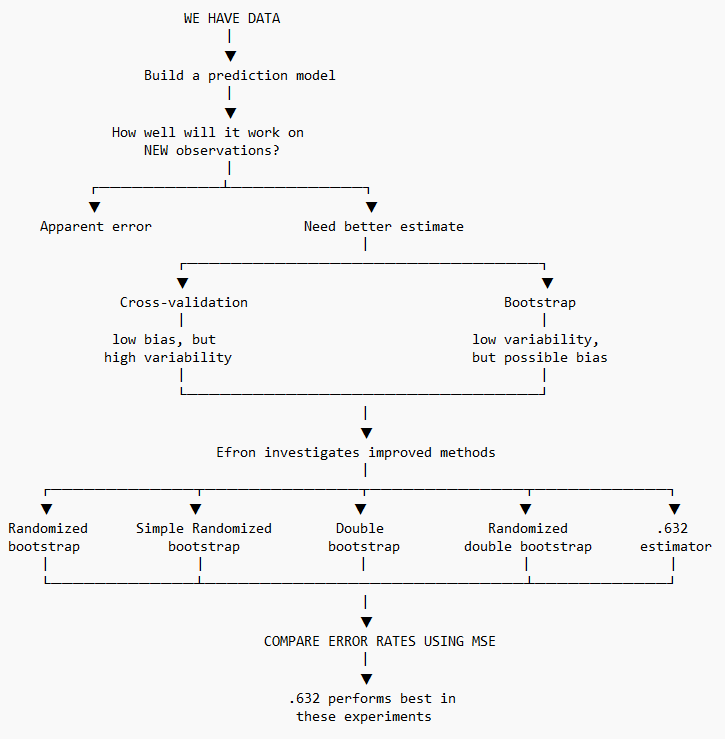
\includegraphics[keepaspectratio]{images/efron-1983-simulation-study-design.png}}

}

\caption{Figure 6: Diagram showing the design for Efron's simulation
study.}

\end{figure}%

\section{Student Simulation of Sampling Experiment
(2,14)}\label{student-simulation-of-sampling-experiment-214}

\subsection{Student Presentation Plan:}\label{student-presentation-plan}

\begin{enumerate}
\def\labelenumi{\arabic{enumi}.}
\tightlist
\item
  I will replicate one of the simulation experiments from Efron's paper,
  focusing on the (2,14) experiment. In this experiment, Efron considers
  a prediction problem with two predictor variables and a training
  sample of 14 observations.
\item
  I will generate data according to the simulation setup described in
  the paper for the (2,14) sampling experiments which used a bivariate
  normal probability model with two predictor variables and two classes.
\item
  Similar to Efron, I will conduct 100 trials of sampling experiment
  (2,14) which will geenerate 100 artificial datasets.
\item
  I will construct the prediction rule using the FIsher's Linear
  Discriminant.
\item
  I will evaluate the apparent error rate to use as a baseline for my
  comparisons.
\item
  I will then estimate its error rate using the leave-one-out cross
  validation, ordinary bootstrap, double boostrap, and .632 estimator
  methods.
\item
  Similar to Efron, I will conduct 200 bootstrap replications per trial
  for ordinary bootstrapping.
\end{enumerate}

\begin{figure}[H]

{\centering \pandocbounded{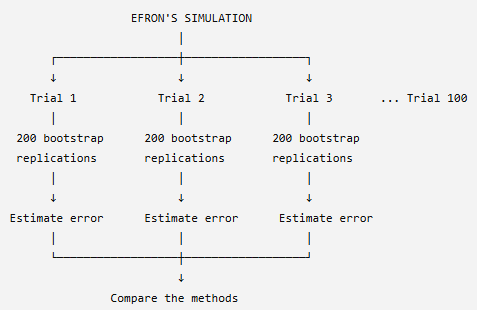
\includegraphics[keepaspectratio]{images/ordinary-bootstrap-replicaiton-per-trial.png}}

}

\caption{Figure 7: Diagram showing the ordrinary bootstrapping process
for the simulation study.}

\end{figure}%

\begin{enumerate}
\def\labelenumi{\arabic{enumi}.}
\setcounter{enumi}{7}
\tightlist
\item
  I will then compare the estimated error rates with the true error rate
  across repeated simulations to investigate how accurately each method
  estimates prediction error. This will be done by calcuating the MSE.
\item
  I will utilize Python as my primary programming lanagauge to complete
  this simulation.

  \begin{itemize}
  \tightlist
  \item
    I will use the numpy package to generate my data and then utilizing
    the sampling experiemnts referenced in the paper to define the
    paremeters for each dataset.
  \item
    I will be using the scikit-learn package to run my various models
    (cross validiaiton, bootstrapping, etc.), create my linea
    rdiscriminant analysis for my prediction rule, and to create my MSE
    for comparing the estimated error rates of each method with the true
    errro rate.
  \item
    I will use scipy to construct statistical equations.
  \end{itemize}
\end{enumerate}

\begin{figure}[H]

{\centering \pandocbounded{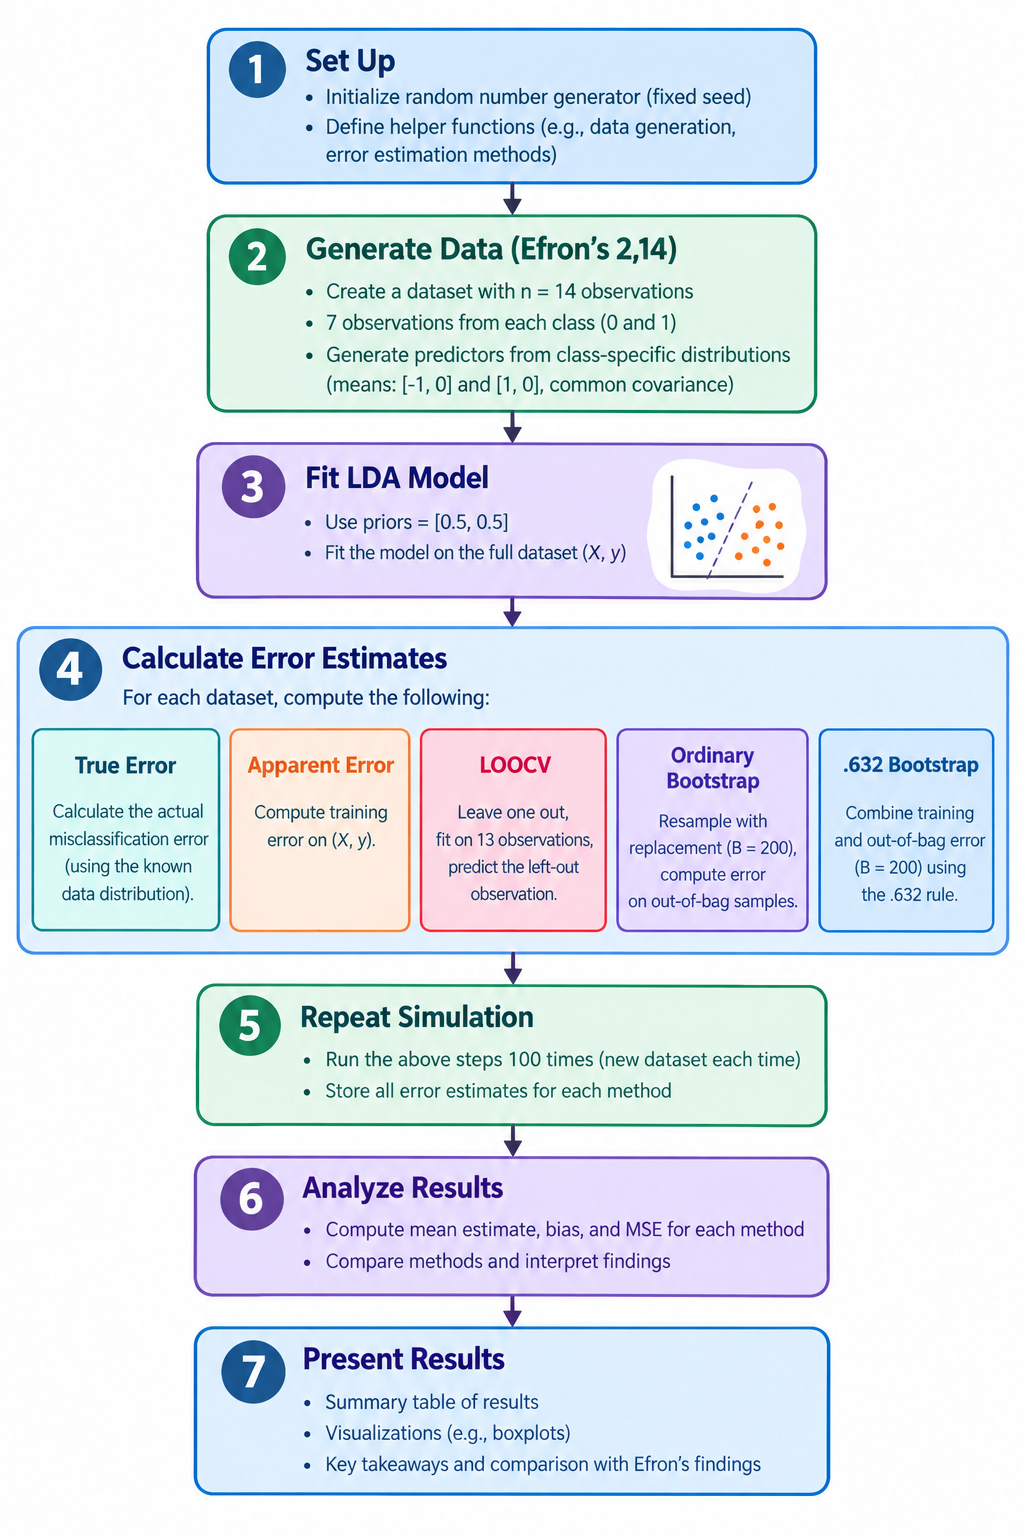
\includegraphics[keepaspectratio]{images/simulation-study-replication-plan.png}}

}

\caption{Figure 8: Diagram showing the design for the simulation study I
am choosing to replicate. The following diagram is using the (2.14)
sampling experiment.}

\end{figure}%

\subsection{Simulation Study Code:}\label{simulation-study-code}

\bookmarksetup{startatroot}

\chapter{imports}\label{imports}

import numpy as np \# import numpy import pandas as pd \# import pandas
import matplotlib.pyplot as plt \# import matplotlib

from scipy.stats import norm \# import normal continuous random variable
from sklearn.discriminant\_analysis import LinearDiscriminantAnalysis \#
import linear discriminant from sklearn.metrics import zero\_one\_loss
\# import zero one classifcation loss (num of misclassifcation) from
sklearn.model\_selection import LeaveOneOut \# import the LOOCV

\bookmarksetup{startatroot}

\chapter{initialize seed for random number
generation}\label{initialize-seed-for-random-number-generation}

rng = np.random.default\_rng(seed=123)

\bookmarksetup{startatroot}

\chapter{create the (2,14) data-generating
function}\label{create-the-214-data-generating-function}

def generate\_214\_data(n=14, rng=None): ``\,``\,'' Generate one dataset
for Efron's (2,14) sampling experiment.

\begin{verbatim}
Parameters
----------
n : int
    Number of observations in the training dataset.
    Efron's (2,14) experiment uses n = 14.

rng : numpy.random.Generator
    Random number generator used for reproducibility.

Returns
-------
X : numpy.ndarray
    Predictor matrix with shape (n, 2).

y : numpy.ndarray
    Binary class labels with shape (n,).
"""

# create a random number generator if one was not provided
if rng is None:
    rng = np.random.default_rng()

# Step 1: Generate class labels.
# Each observation independently has a 50% probability of belonging to either class.
y = rng.binomial(
    n=1,
    p=0.5,
    size=n
)

# Step 2: Create an empty array for two predictors.
X = np.zeros((n, 2))

# Mean vector for Class 0
mean_class_0 = np.array([-1.0, 0.0])

# Mean vector for Class 1
mean_class_1 = np.array([1.0, 0.0])

# Identity covariance matrix
covariance = np.eye(2)

# Step 3: Generate predictor values conditional on class.
for i in range(n):

    if y[i] == 0:
        X[i] = rng.multivariate_normal(
            mean=mean_class_0,
            cov=covariance
        )

    else:
        X[i] = rng.multivariate_normal(
            mean=mean_class_1,
            cov=covariance
        )

return X, y
\end{verbatim}

\bookmarksetup{startatroot}

\chapter{generate dataset}\label{generate-dataset}

X, y = generate\_214\_data( n=14, rng=rng )

\bookmarksetup{startatroot}

\chapter{Class-conditional bivariate normal
distribution}\label{class-conditional-bivariate-normal-distribution}

\begin{itemize}
\tightlist
\item
  The simulated dataset generates binary classes with equal probability
  of 50\% each:

  \begin{itemize}
  \tightlist
  \item
    \(P(Y = 0) = P(Y = 1) = 0.5\) Where predictor vectors follow
    class-conditional bivariate normal distributions:
  \item
    \(X \mid Y=0 \sim \mathcal{N}_2((-1,0)^T, \mathbf{I})\)
  \item
    \(X \mid Y=1 \sim \mathcal{N}_2((1,0)^T, \mathbf{I})\)
  \end{itemize}
\item
  Equal Priors: \(P(Y = 0) = P(Y = 1) = 0.5\)

  \begin{itemize}
  \tightlist
  \item
    What it means: There are two groups/classes in your dataset: Class 0
    and Class 1.
  \item
    Plain English: You have an equal 50/50 chance of picking a point
    from Class 0 or Class 1 (like flipping a fair coin).
  \end{itemize}
\item
  Predictor Vectors: \(X = (X_1, X_2)\)

  \begin{itemize}
  \tightlist
  \item
    What it means: Every single observation (data point) has two
    measurable features/variables, which you can plot as an \((x, y)\)
    point on a standard 2D graph.
  \item
    Plain English: Instead of predicting something based on a single
    number, the model looks at a coordinate pair on a 2D plane to decide
    if it belongs to Class 0 or Class 1.
  \end{itemize}
\item
  Class-Conditional Normal Distributions:
  \(\mathcal{N}_2(\boldsymbol{\mu}, \mathbf{I})\)

  \begin{itemize}
  \tightlist
  \item
    What it means: The data points for each class form a rounded,
    bell-curve-shaped ``cloud'' or cluster around a central center point
    (mean vector \(\boldsymbol{\mu}\)).
  \item
    Mean centers (\(\boldsymbol{\mu}\)):

    \begin{itemize}
    \tightlist
    \item
      Data points for Class 0 cluster around the point \((-1, 0)\) on
      the graph.
    \item
      Data points for Class 1 cluster around the point \((1, 0)\) on the
      graph.
    \end{itemize}
  \item
    Identity Covariance Matrix (\(\mathbf{I}\)):

    \begin{itemize}
    \tightlist
    \item
      The two features \(X_1\) and \(X_2\) are independent of each other
      (non-correlated).
    \item
      The variance (spread) is 1 in all directions.
    \item
      Plain English: The data points spread out equally in every
      direction, creating two neat, circle-shaped clouds of dots
      centered at \((-1, 0)\) and \$(1, 0
    \end{itemize}
  \end{itemize}
\item
  Visualizing the Setup - Imagine a 2D scatter plot:

  \begin{itemize}
  \tightlist
  \item
    You place a target at \((-1, 0)\) for Class 0 (e.g., blue dots) and
    throw darts around it.
  \item
    You place another target at \((1, 0)\) for Class 1 (e.g., red dots)
    and throw darts around it.
  \item
    Because the distance between \(-1\) and \(1\) is only \(2\) units,
    the two clouds of dots overlap in the middle near \(x = 0\).
  \item
    Fisher's Linear Discriminant Analysis (LDA) tries to draw a straight
    line right down the middle (around \(x = 0\)) to separate the blue
    dots from the red dots as accurately as possible.
  \end{itemize}
\end{itemize}

\bookmarksetup{startatroot}

\chapter{Cross Validation}\label{cross-validation-1}

\begin{itemize}
\item
  In a Cross Validation:

  \begin{itemize}
  \tightlist
  \item
    The specific machine learning model is trained using the training
    data.
  \item
    The trained machine learning model is then tested/evaluated using
    testing data which is the data it did not train on.
  \item
    \textbf{IMPORTANT NOTE:}

    \begin{itemize}
    \tightlist
    \item
      Seeing how the model works on data it was not been trained on
      allows us to evaluate how well the model performed. So, within
      each iteration, the same data used to train the model should not
      be used to test that version of the model.
    \item
      Therefore, the data needs to be split into a training dataset and
      a testing dataset.
    \end{itemize}
  \end{itemize}
\item
  For example, in a 4-fold cross valdiaiton, we divide a dataset up into
  4 equally sized folds. We may choose to use the first 75\% of the data
  (first 3 folds of data) to train a particular machine learning model
  then use the last 25\% of the data (last fold of the data) to test the
  machine learning model. However, how do we know if this selection of
  data is the best option? what if using the first 25\% of the data for
  testing the model and the last 75\% for training the model is better?

  {\def\LTcaptype{none} % do not increment counter
  \begin{longtable}[]{@{}ccccc@{}}
  \toprule\noalign{}
  Iteration & Fold 1 & Fold 2 & Fold 3 & Fold 4 \\
  \midrule\noalign{}
  \endhead
  \bottomrule\noalign{}
  \endlastfoot
  1 & Train & Train & Train & \textbf{Test} \\
  2 & Train & Train & \textbf{Test} & Train \\
  3 & Train & \textbf{Test} & Train & Train \\
  4 & \textbf{Test} & Train & Train & Train \\
  \end{longtable}
  }
\item
  Cross validation helps identify and evaluate overfitting by using
  various combinations of data folds for training the model and keeps
  track of how well the model performed using the corresponding testing
  data folds. So, instead of splitting a dataset just once into a
  training set and a testing set, cross validation repeats the process
  multiple times.

  \begin{itemize}
  \tightlist
  \item
    \textbf{IMPORTANT NOTE:}

    \begin{itemize}
    \tightlist
    \item
      Model overfitting is a modeling error that occurs when a machine
      learning model matches its training data too closely, which leads
      it to simply memorizing the data, random noise, and minor quirks
      instead of actually learning from the data to idenfity meaningful,
      true, general patterns.
    \item
      Cross validation can help address overfitting concerns by
      providing a reliable estimate of how well a model performs on
      unseen data rather than just memorizing the training set.
    \end{itemize}
  \end{itemize}
\end{itemize}

\bookmarksetup{startatroot}

\chapter{Bootstrapping}\label{bootstrapping-1}

\begin{itemize}
\tightlist
\item
  The statisics for each of the bootstrapped datasets are taken. This
  could include the mean, median, standard deviation, etc.
\item
  For simplicity, lets assume we are only considering the mean of each
  of the boootstrapped datasets. After collecting all the means for all
  bootstrapped datastes. These means can be plotted onto a histogram
  which is used to visualize the frequency of a particular measurment or
  statistic.
\item
  This histogram which is a distribtuion of bootstrap statisics, in our
  case, distribution of bootstrap means, gives us an idea of how much
  our statistic might vary if we could repeatedly obtain new samples
  from the same population.
\item
  This histrogram can also provide insight into the liklihood of getting
  something close to the original statisic, in our case the mean, of the
  original dataset when the experiment is rerun multiple times by
  looking at the distribution of the histrogram.
\item
  The standard deviation of the bootstrap distribution of the statistic
  from the histogram provides an estimate of the standard error of that
  statistic of the original dataset.
\item
  We can also determine a bootstrap confidence interval which can be
  constructed from the distribution of bootstrap estimates. For example,
  a 95\% bootstrap confidence interval provides a range of plausible
  values for the population parameter based on the bootstrap
  distribution where The interval contains 95\% of the bootstrap
  estimates.
\item
  This can allow us to conduct a hypothesis test to determine whether we
  reject or fail to reject the nu,ll hypothesis.
\end{itemize}

\bookmarksetup{startatroot}

\chapter{Summary}\label{summary}

In summary, this book has no content whatsoever.

\bookmarksetup{startatroot}

\chapter*{References}\label{references}
\addcontentsline{toc}{chapter}{References}

\markboth{References}{References}

\protect\phantomsection\label{refs}
\begin{CSLReferences}{1}{1}
\bibitem[\citeproctext]{ref-Efron1983}
Efron, B. 1983. {``Estimating the Error Rate of a Prediction Rule:
Improvement on Cross-Validation.''} \emph{Journal of the American
Statistical Associati} 78 (382): 316--31.
\url{https://doi.org/10.2307/2288636}.

\bibitem[\citeproctext]{ref-knuth84}
Knuth, Donald E. 1984. {``Literate Programming.''} \emph{Comput. J.}
(USA) 27 (2): 97--111. \url{https://doi.org/10.1093/comjnl/27.2.97}.

\end{CSLReferences}




\end{document}
